\documentclass[12pt, a4paper]{article} 
\usepackage{lmodern}
\usepackage[utf8]{inputenc} %reconhece acentuação
%\usepackage[english,brazil]{babel}
\usepackage[english]{babel}
\usepackage[T1]{fontenc}    %acentuacao
\usepackage{indentfirst}		% Indenta o primeiro parágrafo de cada seção.
\usepackage[left=3.00cm, right=2.00cm, top=2.00cm, bottom=3.00cm]{geometry}
\usepackage{lmodern}			% Usa a fonte Latin Modern
%\usepackage{times} %times new roman font latex command
\usepackage{color}				% Controle das cores
\definecolor{maroon}{RGB}{153, 0, 0}   %cor vermelha nas citacoes
\usepackage[colorlinks=true, linkcolor= black, citecolor=maroon,urlcolor=blue]{hyperref}
\usepackage[pdftex]{hyperref}  %para adicionar enderecos de internet






% Tamanho da pag:
\usepackage{geometry}
\geometry{
	a4paper,
	total={170mm,257mm},
	left=20mm,
	top=20mm,
}

% Espaçamento entre  parágrafos:
\setlength{\parskip}{0.1cm}
% espaçamento entre linhas:
\usepackage{setspace}
\onehalfspacing

% para melhorias de justificação:
\usepackage{microtype} 
% linhas de tabela mais bem feitas
\usepackage{booktabs}

% adicionar nota de rodape nas tabelas
\usepackage{threeparttable}
\usepackage{tablefootnote}

% adicionar nota nas figuras
\usepackage[capposition=top]{floatrow}

% comentar whole section
\usepackage{verbatim}


\usepackage{color,graphicx}
\usepackage{amsthm}
\usepackage{amsmath}
\usepackage{authblk}
\usepackage{amsthm}
\usepackage{amssymb, bm}
\usepackage{dsfont, mathtools}

\usepackage{lmodern}
\usepackage[natbibapa]{apacite} 
\usepackage[hyphens,spaces]{url} 
\usepackage[colorlinks,citecolor=red,urlcolor=blue]{hyperref}

\usepackage{float}

% Abreviação de alguns comandos que uso
%principalmente p fazer notas de aula

\DeclareMathOperator*{\argmax}{arg\!\max}
\DeclareMathOperator*{\argmin}{arg\!\min}
\DeclareMathOperator*{\E}{\mathbb{E}}
\DeclareMathOperator*{\V}{\mathbb{V}}
\DeclareMathOperator*{\C}{\mathbb{C}}
\DeclareMathOperator*{\R}{\mathbb{R}}
\DeclareMathOperator*{\N}{\mathbb{N}}
\DeclareMathOperator*{\B}{\mathcal{B}}
\DeclareMathOperator*{\1}{\mathds{1}}
\DeclareMathOperator*{\bh}{\widehat{\beta}}
\DeclareMathOperator*{\ah}{\widehat{\alpha}}
\DeclareMathOperator*{\>p}{\xrightarrow{p}}
\DeclareMathOperator*{\<p}{\xrightarrow{p}}
\DeclareMathOperator*{\ve}{\varepsilon}
\DeclareMathOperator*{\e}{\epsilon}
\DeclareMathOperator*{\nn}{\nonumber}
\DeclareMathOperator*{\bu}{\bar{u}}
\DeclareMathOperator*{\ulw}{\underline{w}}
\DeclareMathOperator*{\olw}{\overline{w}}



\usepackage{bookmark}
\bookmarksetup{numbered}
\title{Measuring the Natural Rate of Interest in Brazil and identifying its drivers: a DSGE Perspective}
\author{Renan Santos Alves (FGV-EESP)}	\begin{document}
\setlength{\parindent}{1cm} %tamanho do espaçamento de paragro

%%%%%%%%%%%%%     Capa       %%%%%%%%%%%%%%%%%

	\begin{titlepage}
	\begin{center}
		\vspace*{1cm}
		
		\Large 
	Fundação Getúlio Vargas - Escola de Economia de São Paulo 
	
	
		
		\vspace{4cm}
		
	    Projeto de Doutorado em Economia 
		
		\vspace{2cm}
		
		
		\textbf{Measuring the Natural Rate of Interest in Brazil and identifying its drivers: a DSGE Perspective}
		
		\vspace{1cm}
		\normalsize	
	
		\vspace{2cm}
	
	Projeto de Tese de Doutorado Apresentado à Fundação de Amparo à Pesquisa do Estado de São Paulo (Fapesp) para fins de pleito de bolsa de doutorado
	\\	\vspace{1cm}
		Aluno: Renan Santos Alves
		\\
		\vspace{1cm}
		Orientador: Marcel Bertini Ribeiro

	
		

		\normalsize
		\vspace{4cm}
		São Paulo\\
	2021
	\end{center}
	
\end{titlepage}


%%%%%%%%%%%%%     Abstract        %%%%%%%%%%%%%%%%%


\begin{abstract}
	This project proposes to estimate the natural interest rate for Brazil, through a medium-scale New Keynesian open economy dynamic stochastic general equilibrium (DSGE) model using Bayesian techniques on Brazil data to answer the following questions: (i) what the level of Brazil’s natural interest rate between 1999 and 2019; (ii) whether the natural rate has also declined as well as in advanced economies; (iii) what are the mechanisms that explain the Brazilian natural rate; (iv) whether international shocks are fundamental to explain the equilibrium rate.  \\
    \\
    \noindent
	\textbf{Keywords:} Natural Rate of Interest, Monetary Policy, Open Economy, Bayesian Estimation, Business Cycle


\end{abstract}
\thispagestyle{empty}

%%%%%%%%%%%%%     Sumario         %%%%%%%%%%%%%%%%%

%\newpage
%\thispagestyle{empty}
%\tableofcontents

%%%%%%%%%%%%%    Começando projeto        %%%%%%%%%%%%%%%%%

%\newpage
\setcounter{page}{1}
\onehalfspacing

\section{Introduction, Justification and Intention}
The interest rate is the most important instrument of monetary policy. The policymakers to assess monetary policy stance monitor what we call the natural rate of interest . The natural rate of interest  is the real interest rate at which the output is equal to its potential level, and prices neither accelerate nor decelerate. Therefore, the natural rate is a benchmark, since when it is above real interest, monetary policy was contractionary, and when it is below real interest, it was expansionary. The difficulty in monitoring this interest rate is that it cannot be observed and so it must be estimated. 

A decade later, the international financial crisis, the world economy remains sunk in a low interest rate environment amid the unconventional monetary policies implementation promoted by advanced economies, which drew attention to the natural rate of interest . The literature also found evidence for a historical decline and even negative levels in the natural rate in advanced economies over the last two decades, according to \citet{HLW:2017}, \citet{Wynne:2018}, and \citet{DelNegro:2019}.\footnote{\citet{HLW:2017}, using a semi-structural model, and \citet{DelNegro:2019}, through an autoregressive vector (VAR), both find a downward trend in natural rates for advanced economies. \citet{Wynne:2018} find the same result for a larger set of countries. }  
This economic environment is called secular stagnation, as \citet{Summers:2014} characterized it, because of low interest rates and low growth. Some studies to explain the reasons for the fall in interest rates, such as preferences for safe assets \citet{Caballero:2017} and demographic causes \citet{Eggertsson:2019}.

The unconventional monetary policy strategies adopted by the advanced economies in response to the international financial crisis provoked a flood of capital flow towards the emerging economies. The result was rapid credit growth, which has required many emerging countries to adjust their monetary policy to reduce the risks of financial instability and volatility in capital flow. This raises major concerns for policymakers because the capital flow affects the business cycle in emerging countries, \citet{Uribe:2016} and \citet{Cuadra:2019}. 


There are few studies that have investigated the effects of capital flow on the  natural rate in emerging markets. \citet{Carrillo:2018} examine how Mexico's capital flow explains the drop in the natural rate of interest  after the global financial crisis. It is already known that international interest and country spread shocks are drivers of business cycles in emerging economies, according to \citet{Uribe:2006}. These international factors are also important to explain the natural rate in emerging markets. \citet{Barbosa:2016} showed that the Brazilian natural rate could be explained by the international real interest rate and the country risk premium. 


%A stylized fact of the Brazilian economy was the high real interest rate. \citet{SEGURA-UBIERGO:2012} lists some arguments that try to explain why, for many years, Brazil's real interest was higher compared to that of other emerging countries. The combination of high levels of public debt and the fear of a possible default resulted in higher interest rates and an increased risk premium. The low savings rate is a limiting factor for economic growth and, therefore, a reason for higher interest rates. Third, the institutional weakness that creates legal uncertainty by not protecting investors. The presence of public banks offering credit at below-market rates affects the transmission mechanism of monetary policy since the rest of the economy's equilibrium interest rate needs to be higher to keep credit demand under control at a level consistent with the inflation targeting regime.

Brazil's monetary policy is often cited as excessively conservative, evidenced by one of the highest real interest rates among emerging economies. \footnote{A stylized fact of the Brazilian economy was the high real interest rate. \citet{SEGURA-UBIERGO:2012} lists some arguments that try to explain why, for many years, Brazil's real interest was higher compared to that of other emerging countries: The combination of high levels of public debt and the fear of a possible default, the low savings rate is a limiting factor for economic growth, the institutional weakness that creates legal uncertainty by not protecting investors and the presence of public banks offering credit at below-market rates affects the transmission mechanism of monetary policy.} However, as shown in figure 1, Brazil's real interest rate has shown a downward trend in the last 20 years (figure on the left). The lowest real interest level was observed in December 2019, while the highest value was observed in July 1999. One reason why economists justify that Brazilian real interest rates were high is the high rate of inflation and volatility. Brazil adopted the inflation targeting regime in June 1999, and, as shown in the figure on the right, we can see that the inflation rate, measured by the consumer price index, was within the band for most of the years.\footnote{In January 1999, Brazil adopted the floating exchange rate regime, following emerging countries' trends at that time. Between the end of 2002 and the beginning of 2003, with the presidential election and the insecurity of adopting controversial economic measures, the country's risk increased, and the interest rate accompanies this movement.}


\begin{figure}[H]
\centering
\caption{Real interest and inflation in Brazil}
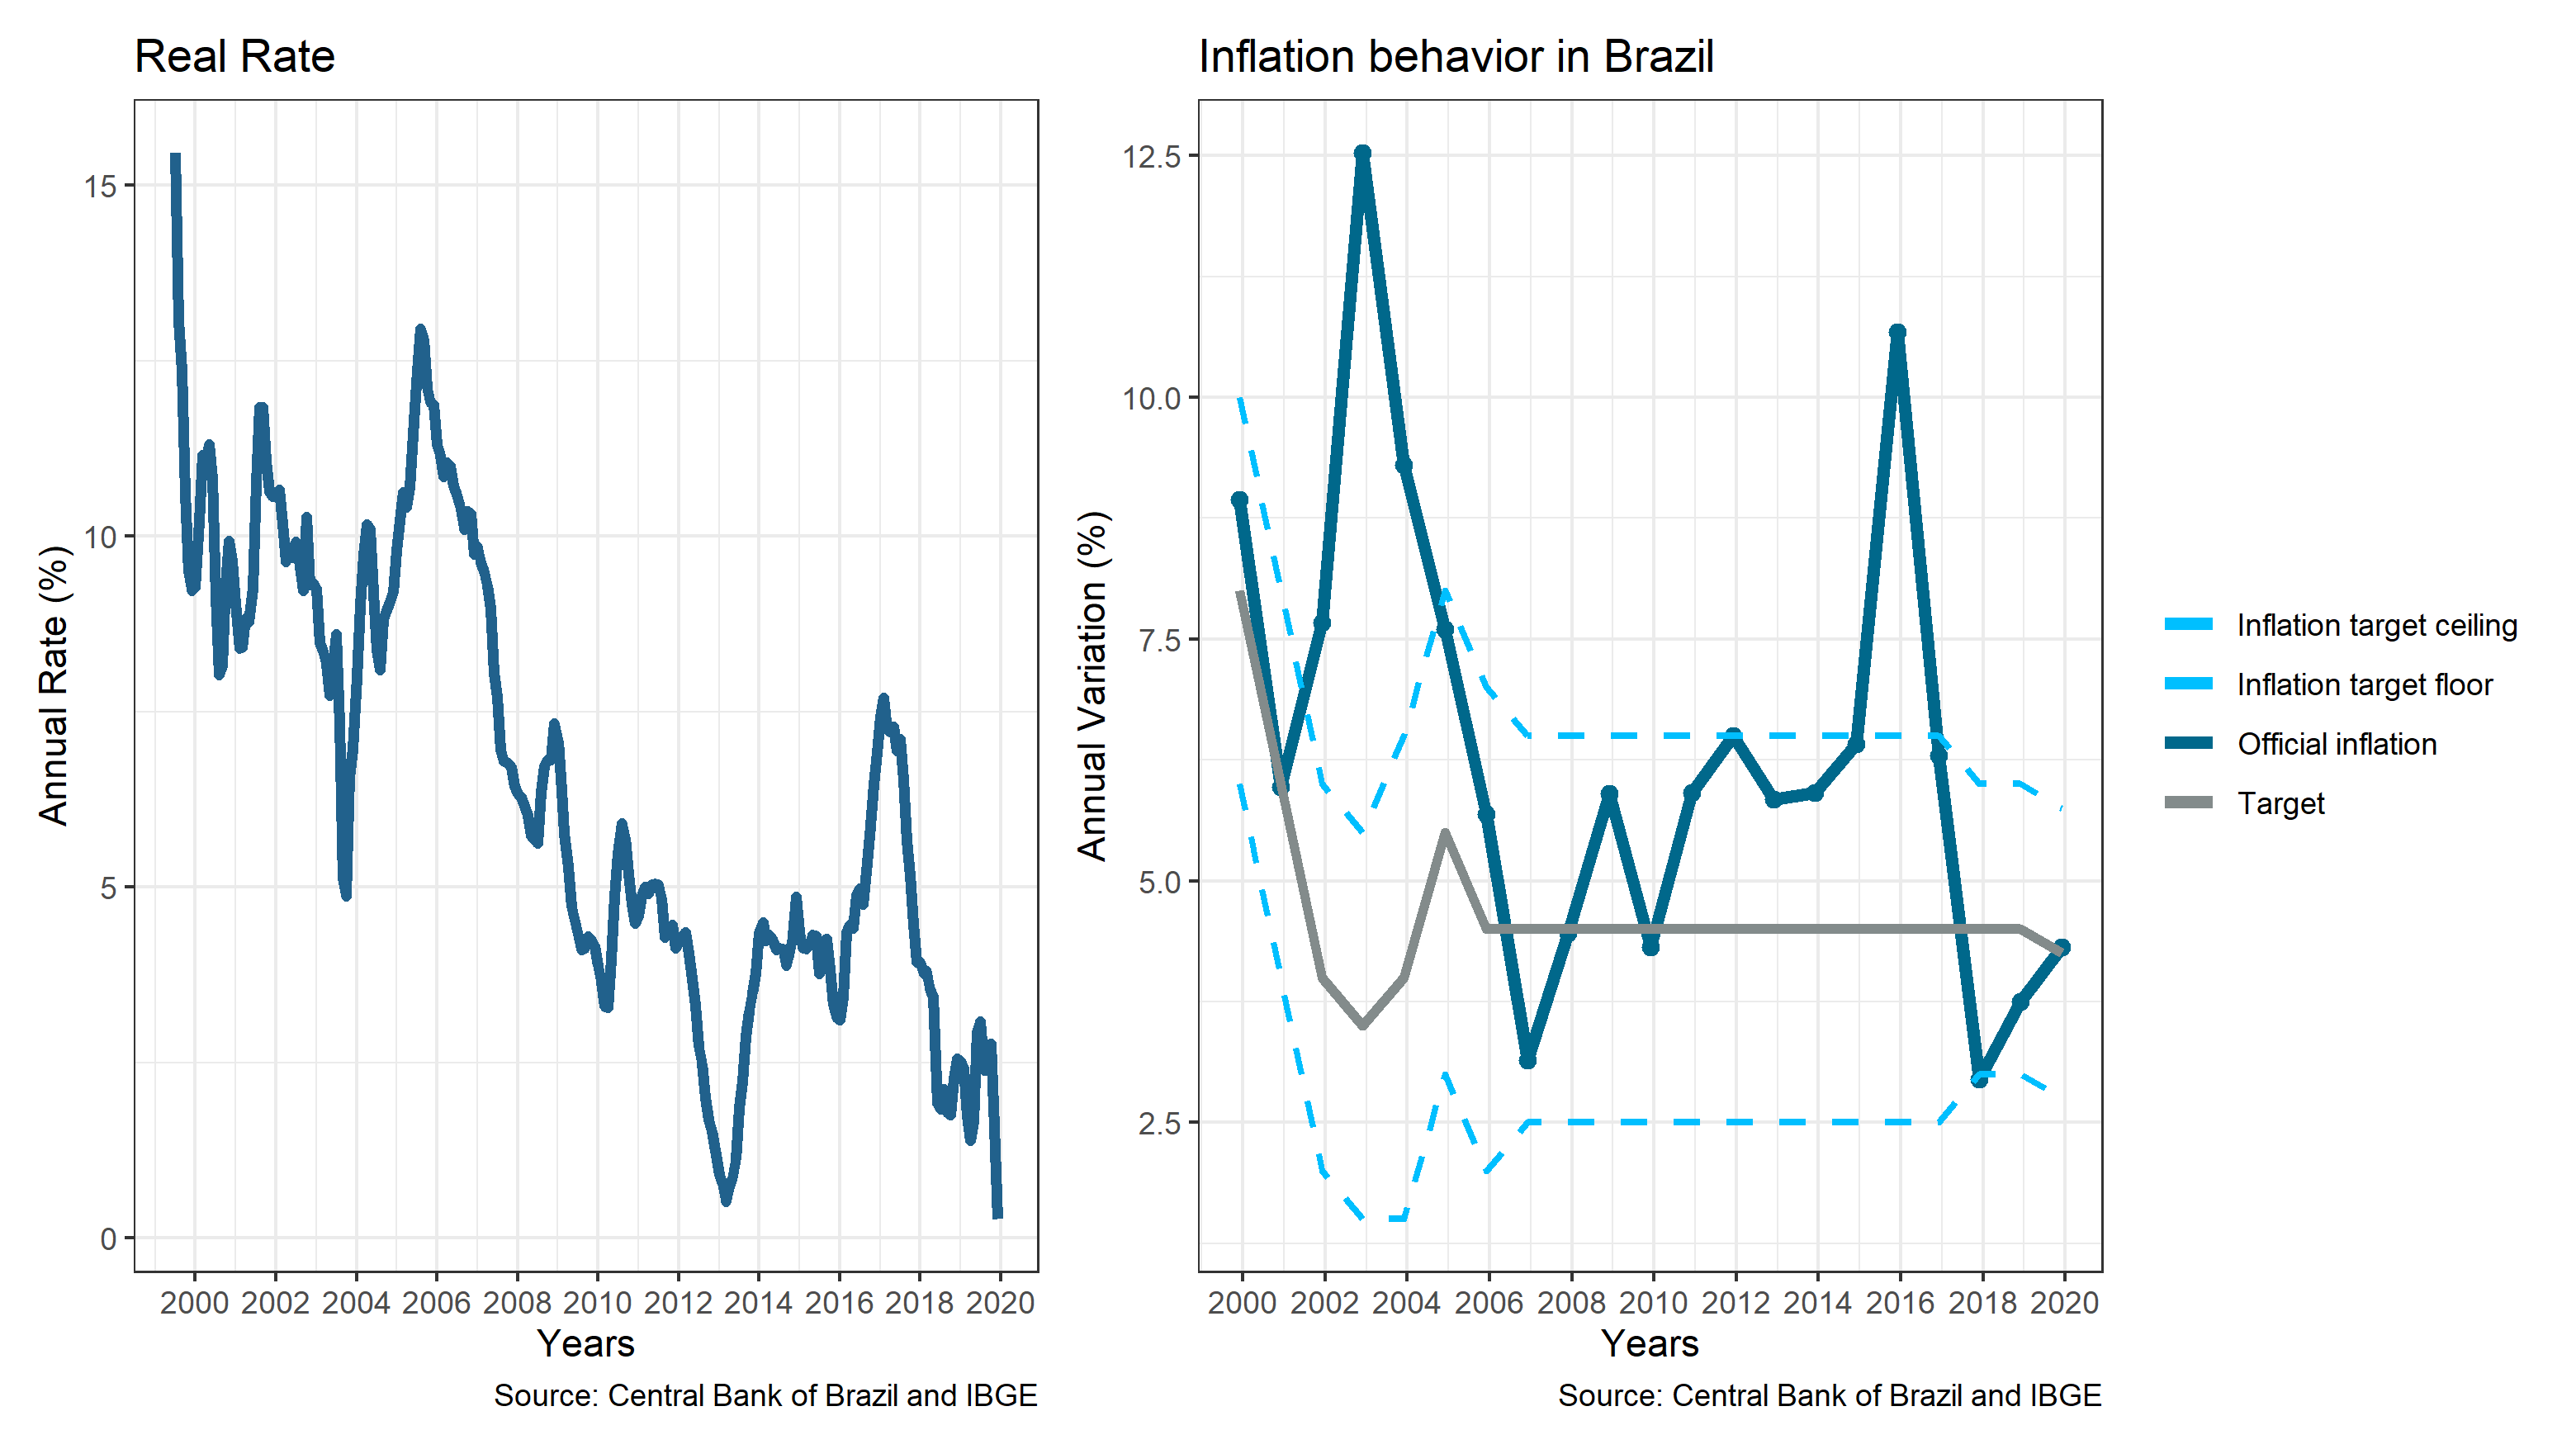
\includegraphics[scale=0.70]{Projeto Fapesp/Juros_inflacao.png}

\end{figure}



%Given this scenario in which interest rates in advanced economies are stuck in the zero lower bound, the emerging economies suffer from international interest rate and risk premium shocks and the fall in real rates in Brazil reaching the lowest level in 20 years, in this paper I estimate an open economy DSGE model based on \citet{Adolfson:2007} to answer the following questions: (i) what the level of Brazil's natural rate of interest  between 1999 and 2019; (ii) is will the natural rate have also declined as well as in advanced economies; (iii) what are the mechanisms that explain the Brazilian natural rate; (iv) whether external shocks are fundamental to explain the balance interest. According to \citet{Woodford:2003}, the natural rate of interest is the interest rate that would prevail if all prices and wages were flexible.

Given this secular stagnation scenario, represented by a downward trend in the real world interest rate and low growth rates in advanced economies, it is interesting to know whether in emerging economies the natural rate of interest  is also falling and whether this low interest rate global environment contributed to this fall. In this project, I estimate a medium-scale New Keynesian open economy dynamic stochastic general equilibrium (DSGE) model using Bayesian techniques on Brazil data to answer the following questions: (i) what the level of Brazil's natural rate of interest  between 1999 and 2019; (ii) whether the natural rate have also declined as well as in advanced economies; (iii) what are the mechanisms that explain the Brazilian natural rate; (iv) whether international shocks are fundamental to explain the equilibrium rate. I follow \citet{Woodford:2003}, the natural rate of interest corresponds to the value of the real interest rate that would be realized if prices and wages are flexible, and absent shocks to the mark-ups on goods and labor markets.



%Few studies investigate whether the natural rate has also fallen in emerging countries, given this scenario in which interest rates in advanced economies have reached the lower limit of zero, and many papers have found evidence for the fall in natural interest in these countries.



I use a structural (DSGE) model in the same way as \citet{Neiss:2003} because this is an approach that has the advantage of providing an economic insight into the drivers of the natural rate. The model used in the analysis is a small open economy follows closely \citet{Adolfson:2007}, which is an extended open economy version of \citet{Christiano:2005} with both nominal and real frictions and \citet{Altig:2011}, who introduce a stochastic unit-root technology shock, which enables me to work with trending data.\footnote{It is a medium-scale version of the open economy models such as \citet{Gali:2005}, \citet{Monacelli:2005} and \citet{Lubik:2007}.} However, the model differs from \citet{Adolfson:2007} in three aspects.\footnote{This DSGE model, called RAMSES, used to forecasting and policy analysis at the Sveriges Riskbank.} First of all, households do not receive utility from holding cash. Second, I allow inflation in Brazil to be higher than inflation in the rest of the world. This allows for a differential in inflation rates, causing a depreciation of the nominal exchange rate at a steady state, which is in line with that predicted by the purchasing power parity theory. Finally, the role of fiscal policy is disregarded in this model.

The central bank's decision to raise or lower the short-term interest rate may have a material effect on the economy. This decision may affect inflation, unemployment, exchange rates and output growth. Due to the importance of setting interest rate, understanding where the natural rate is vital to making effective policy decisions. This becomes even more relevant for the Brazilian economy, given the enormous challenges and uncertainties arising from the fiscal issue, the local political scenario and international factors.

I should note, however, that DSGE models generally estimate the business-cycle frequency component in the natural rate of interest . This is different from pure time-series models and from the semi-structural methods that, in turn, focus on low-frequency movements of the natural rate. However, the existing studies in the DSGE literature tend to
estimate the natural rate of interest  within a closed-economy setup and only for large economies such as the
U.S., the euro area, and Japan.

To my knowledge, my paper is the first attempt to investigate explicitly  the determinants of open economy on the natural rate of interest , in an emerging economy (e.g. Brazil), using a well-structured medium-scale open economy DSGE model, according to \citet{Adolfson:2007}. The model is characterized by nominal frictions, real frictions, incomplete exchange rate pass-through in both the import and export sector by including nominal price rigidities, including stationary and stochastic unit root technology shocks and a larger set of structural shocks, mainly due to the open economy aspects of my model.

%
%
\section{Literature Review}
In the past two decades, various papers have proposed approaches to estimate the unobservable natural rate of interest . This literature can be broadly divided into three strands, following \citet{Giammarioli:2004}: pure time series methods, semi-structural econometrics methods and structural methods.\footnote{For a useful review of the results found in the literature, see \citet{Brand:2018}. } It is worth mentioning that according to \citet{Wieland:2018}, there are three different concepts of the natural rate and this differentiation depends on the time horizon, short-term, medium-term and long-term.\footnote{The first concept of equilibrium rate refers to that of short-term equilibrium and is often used in DSGE models. The second concept of the neutral interest rate in the medium-term, used in the semi-structural models introduced by \citet{LW:2003}. And the third concept is the long-term steady state equilibrium rate. In DSGE models, the long-term neutral rate is the interest at which the short-term rate will converge at a steady state.}

The first approach is through time series methods, such as univariate local level models, multivariate models, time-varying vector autoregression model, and trend-cycle decomposition.\footnote{\citet{DelNegro:2019} use a VAR to understand the dynamics of interest rates in seven advanced economies since 1870, and the natural rate is inferred through a spectrum of bond returns with a trend-cycle approach. \citet{Johannsen:2018} a more flexible time series model, but using a shadow rate measure, which refers to the nominal interest rate would prevail if there were no zero lower bound (ZLB). \citet{Hamilton:2016} analyze the potential drivers of the natural rate; for this, they define the neutral rate as the real long-term rate; they also extract country-by-country trends. \citet{Lubik:2015} uses a simple time-varying parameter vector autoregresion model with  for three variables in the US economy (output growth, inflation, and real interest) to estimate the neutral rate. The natural interest measure is the long-term conditional forecast of the real rate. \citet{Rudebusch:2019} estimates an affine term structure model to capture macroeconomic variables and extract natural interest; they estimate real interest from financial market data. } The time-series approach provides little policy information about the neutral rate's future. The estimates are inaccurate, and the identification hypotheses are not based on theory or non-structural. Compared to the other two approaches, it tends to impose fewer restrictions, and the results of the estimates are more flexible.

The second approach is the semi-structural, and it is also the concept of the medium-term natural rate. This approach started with \citet{LW:2003}’s pioneering work, has received a lot of attention, and has motivated great literature since then.\footnote{ 
\citet{Wu:2007}, \citet{Clark:2005}, \citet{Kiley:2015}, \citet{Juselius:2017}, for the US; \citet{Renne:2007} for the euro area, \citet{Wynne:2018} for the world.} The semi-structural econometrics models combine atheoretical time series methods and a simple Keynesian model, consisting of a relationship between aggregate demand and a Phillips curve.\footnote{The natural rate of interest  is inferred from the structural relationships that link the output gap, inflation, and the deviation of the real interest rate from its natural level implied by an empirical IS curve and an empirical Phillips curve.} The equilibrium interest rate is a latent variable, which depends on the trend growth rate of potential output, some preference parameters, and a unit root process that captures other determinants. More recently, \citet{HLW:2017} updated the United States estimates, based on the \citet{LW:2003} model, and extended the estimate to the Euro area, Canada, and the United Kingdom. The results obtained show an international movement among the natural rate estimates in a closed economy model. They were suggesting that global factors play an important role in determining equilibrium interest rates.

The extension of the \citet{LW:2003} model from a closed economy to an open economy, aiming to understand how global factors impact the neutral rate, is straightforward. \citet{Berger:2014} studies the effect of the exchange rate on natural interest in Canada. \citet{Wynne:2018} investigates how international factors determine equilibrium interest in a two-country setup for the USA and Japan. Instead of estimating for the whole euro area as done by \citet{Renne:2007}, \citet{Fries:2018} estimate the natural rate for the four largest economies in the euro area (Germany, France, Italy, and Spain) and what allows to link the economy of each country is the trade channel and the productivity channel.


The third approach of the literature, the one our where paper fits in, relies on structural models, which can be either New Keynesian (DSGE) models (\citet{Justiniano:2010}, \citet{Melosi:2015}, \citet{Curdia:2015}, \citet{DelNegro:2017} all for the US; \citet{Hristov:2016} for the euro area; \citet{Neri:2018} for the US and the euro area) or overlapping generation (OLG) models (\citet{Gagnon:2016}, \citet{Ferrero:2016}, \citet{Eggertsson:2019}).\footnote{See for DSGE models \citet{Orphanides:2002}, \citet{Edge:2008}, \citet{Lopez-Salido:2009}, \citet{Bjornland:2011}, \citet{Canzoneri:2015}, \citet{Del-Negro:2015}, also for the US; \citet{Okazaki:2018} for Japan;  \citet{Carrillo:2018} RBC model for Mexico; \citet{Grossman:2019} for Australia, Canada, South Korea, Sweden, Switzerland and the UK. For OLG models \citet{Kara:2016} and \citet{Papetti:2020}.} In the structural approach, the neutral rate concept is a purely short-run equilibrium. The natural rate is influenced by temporary shocks other than monetary policy shocks.\footnote{In DSGE models, the natural rate of interest  is an unobserved variable that can be estimated through a structural model, using a set of macroeconomic data.} Estimates of this natural rate often exhibit greater variability than actual real interest rates, which are influenced by the presence of price rigidities.\footnote{The literature has suggested that the central bank determines interest rates so that real interest reaches the short-term natural rate of interest . Such a policy depends heavily on the model and shocks. The counterpart is that the model is not robust for uncertainty but sensitive to the specifications themselves.}

The DSGE models, if correctly specified, have the advantage over semi-structural models and time series models. The former can capture the short-term behavior of the natural rate interest and its evolution throughout the business cycle, which is the most important for monetary policy.\footnote{It is essential to be careful when interpreting the results since the structural models also suffer from “omitted shock bias.” For this reason, they will divide the disturbances only between the categories consciously built by the researcher.} The second advantage of the DGSE models over the others is the possibility of evaluating optimal monetary policies when the natural rate of interest  varies, see \citet{Gali:2019}. According to \citet{Brand:2018}, the neutral rate estimates in DSGE models are more volatile than in semi-structural models. This diagnosis is because, in semi-structural models, the measure of equilibrium interest is based on a statistical definition of the potential output, which evolves over time. In contrast, in DGSE models, the natural interest estimates are based on its natural product measures, which change according to the shocks that affect the business cycle.\footnote{This volatility is of concern for two reasons. First, policy makers may think that the neutral rate should be very smooth and understand that cyclical changes in neutral interest are due to errors. According to them, they notice a discomfort in relation to the estimates with a relatively low signal-to-noise ratio.}




%%
\section{Schedule}
The present work is planned to last three semesters, starting in the first semester of 2021. Below is the division of activities that will be carried out over the period.
\begin{itemize}
    \item [(1)] \textit{Literature Review}: Reading papers that estimate the neutral interest rate. The literature is divided into three approaches: the first corresponds to time series models, the second to semi-structural models and the third to structural models. The objective at this stage of the project is to understand the approached methodology, to understand the differences between the approaches, both in the construction of the models and in the estimation processes.
    
     
    
    \item [(2)] \textit{Development of the theoretical model}: In this stage, a DSGE model will be adapted for the Brazilian economy, which allows estimating Brazil's natural rate of interest , after the inflation target regime in 1999.
    
    \item [(3)] \textit{Data preparation and organization}: Previous analysis of the time series used, making seasonality corrections and performing basic tests.
    
    \item [(4)]\textit{Data analysis and estimation}: Estimating the Brazilian economy model, testing what the best way to incorporate the desired specificities is. In this step, I will make minor specification adjustments and test the robustness of the model.
    
    \item [(5)] \textit{Results Analysis}: In this step, I analyze the results of the estimates.
    
    \item [(6)] \textit{Final Report and Review}: As a final part of the thesis, I will compile the estimates made and type the article. I will also write a text for FAPESP's final report.
    
\end{itemize}

Below is the table with the schedule to be followed during the project.

\begin{table}[H]
\centering
\caption{Schedule}
\begin{tabular}{|l|l|l|l|}
\hline
                                      & \multicolumn{2}{c|}{2021} & \multicolumn{1}{c|}{2022} \\ \hline
\textbf{Activity}                    & 1S          & 2S          & 1S   \\ \hline
(1) Literature Review             & x           &             &      \\ \hline
(2) Development of the theoretical model & x           & x           &      \\ \hline
(3) Data preparation and organization   & x           &             &      \\ \hline
(4) Data analysis and estimation     & x           & x           & \multicolumn{1}{c|}{x}    \\ \hline
(5) Results Analysis            &             & x           &  \multicolumn{1}{c|}{x}    \\ \hline
(6) Final Report and Review         &             & x           & \multicolumn{1}{c|}{x}    \\ \hline
\end{tabular}
\end{table}




%
%
\section{Data}






The series data used during the project will be extracted from the Central Bank of Brazil, \url{www.bcb.gov.br}, the Brazilian Institute of Geography and Statistics (IBGE), \url{www.ibge.gov.br}, the Institute for Applied Economic Research (IPEA), \url{www.ipeadata.gov.br} and the Federal Reserve Bank (FRED) \url{https://fred.stlouisfed.org/}, and will not incur any additional monetary costs for the research.

We use quarterly Brazilian data for the period  1999:3-2019:4. I have chosen as domestic variables, the GDP, consumption, investment, exports, imports, IPCA inflation, IGPM inflation, nominal short term interest rate, real exchange rate, country risk preimum, hours, and real wages. For the foreign variables, I use GDP, GDP deflator inflation, interest rate.


%
%
\section{The DSGE Model }

The model is an open economy DSGE following the one developed by \citet{Adolfson:2007} and \citet{Adolfson:2008}, which shares the characteristics and extends the new Keynesian models with the closed economy, \citet{Christiano:2005}, \citet{Altig:2011} and \citet{Smets:2003}.

The economic model consist of households, domestic goods firms, importing consumption and investment firms, exporting firms, a government, a central bank, and an exogenous foreign economy. 
The household maximize a utility function consisting of consumption and leisure and exhibit habit formation in consumption. However, in the open economy model, the households consume both domestic and imported goods. Also, following \citet{Erceg:2000}, each household is a monopoly supplier of a differentiated labor service, which implies they can set their own wages.  Wage stickiness is introduced through an indexation variant of the \citet{Calvo:1983} model.

Household can invest in their stock of capital, save in domestic bonds and/or foreign bonds. Changes to the rate of investment are subject to adjustment costs and household can also vary the rate at which capital is utilised, subject to adjustment cost. The choice between domestic and foreign bonds balances into an arbitrage condition pinning down expected exchange rate changes. (i.e. an uncovred interest rate parity condition). Compared to a standard setting the risk premium is allowed to be negatively correlated with the expected change in the exchange rate.

In the model there are three types of firms: domestic producers, importers and exporters. Domestic firms determine the capital and labor inputs used in their production which is exposed to both transitory and permanent technology shocksas in \citet{Altig:2011}. The firms (domestic, importing and exporting) all produce differentiated goods and set prices according to an indexation variant of the Calvo model. By including nominal rigidities in the importing and exporting sectors we allow for short-run incomplete exchange rate pass-through to both import and export prices.

The central bank is assumed to follow a Taylor type rule in setting the short-term policy interest rate. The model adopts a small open economy perspective where we assume that the
foreign economy is exogenous. The foreign inflation, output and interest rate are therefore assumed to be given by an exogenous VAR. 

I present the full loglinear approximation of the model. For a more detailed description of the complete model and the derivation of the loglinear approximation, see \citet{Adolfson:2007}. Hat symbols on variables denote the log-deviations from steady-state values $\left(\hat{X}_t = dX_t/X = lnX_t - lnX  \right)$. Lower-case letters indicate
that variables have been normalised with the
trend level of technology, that is, $x_t = X_t/z_t$.
Variables with no time subscript refer to steady state values.
%%%
%%%
\subsection{Firms}
%%%
\subsubsection{Domestic goods}
Output of intermediate good firm $i$ is given by the following production function:

\begin{equation}
    \hat{y}_{t}=\lambda^{d}\left(\hat{\varepsilon}_{t}+\alpha\left(\hat{k}_{t}-\hat{\mu}_{t}^{z}\right)+(1-\alpha) \hat{H}_{t}\right)
\end{equation}

where $\hat{H}_{t}$ denotes homogeneous labor hired by the $i^{th}$ firm, $\hat{k}_{t}$ is the capital services stock which may differ from the physical capital stock since I allow for variable capital utilization in the model. \footnote{The production function is given by $Y_{i, t}=z_{t}^{1-\alpha} \epsilon_{t} K_{i, t}^{\alpha} H_{i, t}^{1-\alpha}-z_{t} \phi$.} The process for the permanent technology level $z_t$ is exogenously given by:

\begin{equation}
\frac{z_{t}}{z_{t-1}}=\mu_{t}^{z}
\end{equation}

I have used that the log-linearized real rental rate of capital $r_t^{k}$, is given by:
\begin{equation}
    \hat{r}_{t}^{k}=\hat{w}_{t}+\hat{\mu}_{t}^{z} + \hat{R}_t^{f}-\hat{k}_{t}+\hat{H}_{t}
\end{equation}


Nominal domestic prices are governed by \citet{Calvo:1983} contracts, augmented by indexation to the last period’s inflation and the current (domestic) inflation target. The implied inflation dynamics are given by the following Phillips Curve(s):

\begin{equation}
     \begin{aligned}
    \hat{\pi}_{t}^{d}-\hat{\tilde{\pi}}_{t}^{c} &=\frac{\beta}{1+\beta \kappa_{d}}\left(E_{t} \hat{\pi}_{t+1}^{d}-\rho_{\pi} \hat{\bar{\pi}}_{t}^{c}\right)+\frac{\kappa_{d}}{1+\beta \kappa_{d}}\left(\hat{\pi}_{t-1}^{d}-\hat{\tilde{\pi}}_{t}^{c}\right)-\frac{\beta \kappa_{d}\left(1-\rho_{\pi}\right)}{1+\beta \kappa_{d}} \hat{\bar{\pi}}_{t}^{c} \\
    &+\frac{\left(1-\theta_{d}\right)\left(1-\beta \xi_{d}\right)}{\left(1+\beta \kappa_{d}\right) \xi_{d}}\left(\hat{m} c_{t}^{d}+\hat{\lambda}_{t}^{d}\right)
    \end{aligned} 
\end{equation}
   
where $\hat{\tilde{\pi}}_{t}^{c}$, $\hat{m} c_{t}^{d}$ and $\hat{\lambda}_{t}^{d}$ denote the current inflation target, firm´s real marginal cost, and time-varying markup in the domestic goods market, respectively. Parameters $\rho_{\pi}$, $\beta$, $\xi_{d}$ and $\kappa_{d}$ are the persistence of the inflation target shock; the discount factor; the Calvo parameter (i.e. the probability that the firm is not allowed to re-optimise in period t); and the indexation parameter, respectively. If the indexation parameter $\kappa_{d}$ is 0, the Phillips Curve is purely forward-looking; and if $\kappa_{d} = 1$, prices are fully indexed to last period’s inflation.
   
The real marginal cost $\hat{m} c_{t}^{d}$ are given by:

\begin{equation}
\begin{aligned}
\hat{m} c_{t}^{d} &=\alpha \hat{r}_{t}^{k}+(1-\alpha)\left[\widehat{\bar{w}}_{t}+\hat{R}_{t}^{f}\right]-\hat{\varepsilon}_{t} \\
&=\alpha\left(\hat{\mu}_{t}^{z}+\hat{H}_{t}-\hat{k}_{t}\right)+\widehat{\bar{w}}_{t}+\hat{R}_{t}^{f}-\hat{\varepsilon}_{t}
\end{aligned}
\end{equation}

This is derived from firms’ optimal conditions (total payments for capital services should equal costs of hiring labour each period) and the assumption that firms finance part of their wage bill with funds borrowed one period prior (at $\hat{R}_{t-1}$). Marginal cost is also a function of the gross effective nominal rate of interest rate paid by firms $\hat{R}_{t}^{f}$. Finally, $\hat{\mu}_{t}^{z}$ and $\hat{\varepsilon}_{t}$ denote the permanent and stationary technology shocks, respectively.
%%%
\subsubsection{Imported goods}
The import sector consists of firms that buy a homogenous good in the world market. There are two different types of these importing firms; one that turns the imported product into a differentiated consumption good $C_{i,t}^{m}$, and another that turns it into a differentiated investment good $I_{i,t}^{m}$.

The different importing firms buy the homogenous good at price $P_t^{*}$ in the world market. In order to allow for incomplete exchange rate pass-through to the consumption and investment import prices we assume local currency price stickiness. The importing firms follow Calvo price setting and are allowed to change their price only when they receive a random price change signal. \footnote{There would be complete pass-through in the absence of nominal rigidities, since there are neither distribution costs in the import and export sectors nor an endogenous pricing to market behavior among the firms in the model.}

The New Keynesian Phillips curve of imported consumption and investment goods:
\begin{equation}
    \begin{aligned}
    \hat{\pi}_{t}^{m, c}-\hat{\bar{\pi}}_{t}^{c} &=\frac{\beta}{1+\beta \kappa_{m, c}}\left(E_{t} \hat{\pi}_{t+1}^{m, c}-\rho_{\pi} \hat{\bar{\pi}}_{t}^{c}\right)+\frac{\kappa_{m, c}}{1+\beta \kappa_{m, c}}\left(\hat{\pi}_{t-1}^{m, c}-\hat{\bar{\pi}}_{t}^{c}\right)-\frac{\kappa_{m, c} \beta\left(1-\rho_{\pi}\right)}{1+\beta \kappa_{m, c}} \hat{\bar{\pi}}_{t}^{c} \\
    &+\frac{\left(1-\xi_{m, c}\right)\left(1-\beta \xi_{m, c}\right)}{\left(1+\beta \kappa_{m, c}\right) \xi_{m, c}}\left(\hat{m} c_{t}^{m, c}+\hat{\lambda}_{t}^{m, c}\right)
    \end{aligned}
\end{equation}

\begin{equation}
     \begin{aligned}
    \hat{\pi}_{t}^{m, i}-\hat{\bar{\pi}}_{t}^{c} &=+\frac{\beta}{1+\beta \kappa_{m, i}}\left(E_{t} \hat{\pi}_{t+1}^{m, i}-\rho_{\pi} \hat{\bar{\pi}}_{t}^{c}\right)+\frac{\kappa_{m, i}}{1+\beta \kappa_{m, i}}\left(\hat{\pi}_{t-1}^{m, i}-\hat{\bar{\pi}}_{t}^{c}\right)-\frac{\kappa_{m, i} \beta\left(1-\rho_{\pi}\right)}{1+\beta \kappa_{m, i}} \hat{\bar{\pi}}_{t}^{c} \\
    &+\frac{\left(1-xi_{m, i}\right)\left(1-\beta \xi_{m, i}\right)}{\left(1+\beta x_{m, i}\right) \xi_{m, i}}\left(\hat{m} c_{t}^{m, i}+\hat{\lambda}_{t}^{m, i}\right)
    \end{aligned}
\end{equation}

where $\hat{\pi}_{t}^{m, c}$, $\hat{\pi}_{t}^{m, i}$ $\hat{m} c_{t}^{m, c}$, $\hat{m} c_{t}^{m, i}$, $\hat{\lambda}_{t}^{m,c}$, and $\hat{\lambda}_{t}^{m,i}$ denote the imported consumption goods inflation, imported investment goods inflation, importing consumption firm´s marginal cost, importing investment firm´s marginal cost, time-varying markup in the imported consumption goods market, and time-varying markup in the imported investment goods market respectively. The parameters $\xi_{m,c}$ ($\xi_{m,i}$), and  $\kappa_{m,c}$ ($\kappa_{m,i}$) are Calvo import consumption (investment) price and indexation import consumption (investment) parameter, respectively.

The marginal costs for consumption and investment good importers are given by:

\begin{equation}
    \widehat{m c}_{t}^{m, c}=-\widehat{m c}_{t}^{x}-\hat{\gamma}_{t}^{x, *}-\hat{\gamma}_{t}^{m c, d}
\end{equation}

\begin{equation}
    \widehat{m c}_{t}^{m, i}=-\widehat{m c}_{t}^{x}-\hat{\gamma}_{t}^{x, *}-\hat{\gamma}_{t}^{m i, d}
\end{equation}

where $\widehat{m c}_{t}^{x}$ t is the relative price observed by the domestic exporters $\left(P_t/S_tP_t^{x} \right)$; $\hat{\gamma}_{t}^{x, *}$  is the relative price between the domestically produced goods and the foreign goods; and $\gamma_t^{mc,d}$ and $\gamma_t^{mi,d}$ are the
relative prices of imported consumption and investment goods.
%%%
\subsubsection{Exported goods}
The New Keynesian Phillips curve of exported goods:

\begin{equation}
    \begin{aligned}
\hat{\pi}_{t}^{x} - \hat{\bar{\pi}}_{t}^{c} &=\frac{\beta}{1+\beta \kappa_{x}}\left(E_{t} \hat{\pi}_{t+1}^{x}-\rho_{\pi} \hat{\pi}_{t}^{c}\right)+\frac{\kappa_{x}}{1+\beta x_{x}}\left(\hat{\pi}_{t-1}^{x}-\hat{\bar{\pi}}_{t}^{c}\right)-\frac{\kappa_{x} \beta\left(1-\rho_{\pi}\right)}{1+\beta \kappa_{x}} \hat{\bar{\pi}}_{t}^{c} \\
&+\frac{\left(1-\xi_{x}\right)\left(1-\beta \xi_{x}\right)}{\left(1+\beta \kappa_{x}\right) \xi_{x}}\left(\hat{m} c_{t}^{x}+\hat{\lambda}_{t}^{x}\right)
\end{aligned}
\end{equation}

where $\hat{\pi}_{t}^{x}$ and $\hat{\lambda}_{t}^{x}$ denote the exported  goods inflation, and time-varying markup in the exported goods, respectively.

The marginal costs for exported goods:
\begin{equation}
    \hat{m} c_{t}^{x}=\hat{m} c_{t-1}^{x}+\hat{\pi}_{t}^{d}-\hat{\pi}_{t}^{x}-\Delta \hat{S}_{t}
\end{equation}

where $S_t$ is the nominal exchange rate
%%%
\subsection{Households}
Households have habit formation in their preferences (captured by the parameter $b$). Because of this, the marginal utility of consumption depends on current, lagged and expected future
levels of consumption. The equilibrium condition for household consumption, $\hat{c}_t$, is

\begin{equation}
    \begin{aligned}
\hat{c}_{t} &=\frac{\mu^{z} b}{\left(\mu^{z}\right)^{2}+\beta b^{2}} \hat{c}_{t-1}+\frac{\beta \mu^{z} b}{\left(\mu^{z}\right)^{2}+\beta b^{2}} E_{t} \hat{c}_{t+1}-\frac{\mu^{z} b}{\left(\mu^{z}\right)^{2}+\beta b^{2}}\left(\hat{\mu}_{t}^{z}-\beta E_{t} \hat{\mu}_{t+1}^{z}\right) \\
&-\frac{\left(\mu^{z}-b\right)\left(\mu^{z}-\beta b\right)}{\left(\mu^{z}\right)^{2}+\beta b^{2}}\left(\hat{\psi}_{t}^{z}+\hat{\gamma}_{t}^{c, d}\right)+\frac{\mu^{z}-b}{\left(\mu^{z}\right)^{2}+\beta b^{2}}\left(\mu^{z} \hat{\xi}_{t}^{c}-\beta b E_{t} \hat{\zeta}_{t+1}^{c}\right)
\end{aligned}
\end{equation}

Nominal wages are also subject to the Calvo adjustment mechanism, with indexation to the last period’s CPI inflation $\hat{\pi}_{t-1}^c$, the current (domestic) inflation target $\hat{\bar{\pi}}_{t}^c$ and the steady state growth rate of technology (\citet{Adolfson:2007}  assume that wages are indexed to the current realisation of technology; see also \citet{Altig:2011}). This yields an equation for the
real wage $\hat{\bar{w}}$:

\begin{equation}
\label{labor_wage_equation}    \hat{w}_{t}=-\frac{1}{\eta_{1}}\left[\begin{array}{l}
    \eta_{0} \hat{w}_{t-1}+\eta_{2} E_{t} \hat{w}_{t+1}+\eta_{3}\left(\hat{\pi}_{t}^{d}-\hat{\tilde{\pi}}_{t}^{c}\right)+\eta_{4}\left(E_{t} \hat{\pi}_{t+1}^{d}-\rho_{\pi} \hat{\tilde{\tau}}_{t}^{c}\right) \\
    +\eta_{5}\left(\hat{\pi}_{t-1}^{c}-\hat{\tilde{\pi}}_{t}^{c}\right)+\eta_{6}\left(\hat{\pi}_{t}^{c}-\rho_{\pi} \hat{\tilde{\pi}}_{t}^{c}\right)+\eta_{7} \hat{\psi}_{t}^{z}+\eta_{8} \hat{H}_{t}+\eta_{9} \zeta_{t}^{h}
    \end{array}\right]
\end{equation}

where  $\hat{\psi}_{t}^{z}$ and $\xi_{t}^{h}$ denote the  Lagrangian multiplier and labour supply shock, respectively.

Parameters in Equation (\ref{labor_wage_equation}) are defined as follows:
$$b_{w}=\frac{\lambda_{w} \sigma_{L}-\left(1-\lambda_{w}\right)}{\left(1-\beta \xi_{w}\right)\left(1-\xi_{w}\right)},$$

$$
\left(\begin{array}{c}
\eta_{0} \\
\eta_{1} \\
\eta_{2} \\
\eta_{3} \\
\eta_{4} \\
\eta_{5} \\
\eta_{6} \\
\eta_{7} \\
\eta_{8} \\
\eta_{9}
\end{array}\right)=\left(\begin{array}{c}
b_{w} \xi_{w} \\
\lambda_{w} \sigma_{L}-b_{w}\left(1+\beta \xi_{w}^{2} \right) \\
b_{w} \beta \xi_{w} \\
-b_{w} \xi_{w} \\
b_{w} \beta \xi_{w} \\
b_{w} \xi_{w} \kappa_{w} \\
-b_{w} \beta \xi_{w} \kappa_{w} \\
\left(1-\lambda_{w}\right) \\
-\left(1-\lambda_{w}\right) \sigma_{L} \\
-\left(1-\lambda_{w}\right)
\end{array}\right)
$$

where $\xi_w$ is the Calvo wage parameter (i.e. the probability that the household is not allowed to reoptimise its wage); $\lambda_w$ is the wage mark-up; and $\sigma_{L}$ is the elasticity of labour supply.

The equilibrium condition for investment ($\hat{i}_t$) is given by:

\begin{equation}
    \hat{i}_{t}=\frac{1}{1+\beta}\left[\beta E_{t} \hat{i}_{t+1}+\hat{i}_{t-1}+\beta E_{t} \hat{\mu}_{t+1}^{z}-\mu_{t}^{z}\right]+\frac{1}{\left(\mu^{z}\right)^{2} \phi_{i}(1+\beta)}\left(\hat{P}_{t}^{k}-\hat{\gamma}_{t}^{i, d}+\hat{\zeta}_{t}^{i}\right)
\end{equation}

where $\hat{P}_{t}^{k}$ is the hypothetical price of installed
capital; $\hat{\zeta}_{t}^{i}$ denotes the investment-specific technology shock.

The log-linearised first-order condition for the
physical stock of capital, $\bar{k}_t$, is

\begin{equation}
    \hat{P}_{t}^{k}=E_{t}\left[\frac{(1-\delta) \beta}{\mu^{z}} \hat{P}_{t+1}^{k}+\hat{\psi}_{t+1}^{2}-\hat{\psi}_{t}^{z}-\hat{\mu}_{t+1}^{z}+\frac{\mu^{z}-(1-\delta) \beta}{\mu^{z}} \hat{r}_{t+1}^{k}\right]
\end{equation}

where $\delta$ is the rate of depreciation. The Capital’s law-of-motion:

\begin{equation}
    \hat{\bar{k}}_{t+1}=\frac{1-\delta}{\mu^{z}}\left(\hat{\bar{k}}_{t}-\hat{\mu}_{t}^{z}\right)+\left(1-\frac{1-\delta}{\mu^{z}}\right)\left(\hat{i}_{t}+\hat{\zeta}_{t}^{i}\right)
\end{equation}

The degree of capacity utilization (the difference
between the physical capital stock and capital services) $\hat{u}_t$ is given by:

\begin{equation}
     \hat{u}_{t}=\frac{1}{\sigma_{a}} \hat{r}_{t}^{k}
\end{equation}

where $\sigma_{a}$ is the slope of the utilization cost
function. The capital services is

\begin{equation}
    \hat{k}_{t}=\hat{\bar{k}}_{t}+\hat{u}_{t}
\end{equation}


The modified risk premium-adjusted uncovered interest rate parity
condition is given by:

\begin{equation}
    \hat{R}_{t}-\hat{R}_{t}^{*}&=&\left(1-\tilde{\phi}_{s}\right) E_{t} \Delta \hat{S}_{t+1}-\tilde{\phi}_{s} \Delta \hat{S}_{t}-\tilde{\phi}_{a} \hat{a}_{t}+\hat{\tilde{\phi}}_{t}
\end{equation}

Under the specific modelling assumption that the net foreign asset position of the domestic economy ($\hat{a}_t$) and the risk premium shock ($\hat{\tilde{\phi}}_{t}$). The interest rate at which households purchase foreign bonds is adjusted with a risk premium that depends on the domestic economy’s indebtedness in the international asset market. \citet{Uribe:2003}  show that the inclusion of this debt-elastic risk premium is crucial for the determination of a well-defined steady state in small open economy models. 

In addition, following \citet{Adolfson:2008}, we assume that the risk premium is not only a function of the net foreign asset position, but also the expected depreciation of the domestic currency, $S_{t+1}/S_t$. The inclusion of the expected exchange rate in the risk premium aims to account for the “forward premium puzzle”: an empirical anomaly according to which currencies with higher risk premiums \textit{ex ante} often tend to appreciate \textit{ex post}, and hence a negative relationship exists between risk premia and expected depreciations. 
%%%
\subsection{The Central Bank}
Monetary policy is modelled according to the following reaction function:
\begin{equation}
\widehat{R}_{t}=\rho_{R} \widehat{R}_{t-1}+\left(1-\rho_{R}\right)\left(\widehat{\pi}_{t}^{c}+r_{\pi}\left(\hat{\pi}_{t-1}^{c}-\hat{\pi}_{t}^{c}\right)+r_{y} \hat{y}_{t-1}+r_{x} \hat{x}_{t-1}\right)+r_{\Delta \pi} \Delta \hat{\pi}_{t}^{c}+r_{\Delta y} \Delta \hat{y}_{t}+\varepsilon_{R, t}
\end{equation}

where $\widehat{R}_{t}$ is the short-rate interest rate, $\widehat{\pi}_{t}^{c}$ the CPI inflation, $\hat{y}_{t}$ the output, $hat{x}_{t}$ the log-linearized real exchange rate, and a monetary policy shock $\varepsilon_{R, t}$. The CPI inflation
measure is model-consistent but ignores indirect taxes:
\begin{equation}
      \hat{\pi}_{t}^{c}=\left(1-\vartheta_{c}\right)\left(\frac{1}{\gamma^{c, d}}\right)^{1-\eta_{\epsilon}} \hat{\pi}_{t}^{d}+\vartheta_{c}\left(\gamma^{m c, c}\right)^{1-\eta_{c}} \hat{\pi}_{t}^{m, c}
\end{equation}
%%%
\subsection{Relative prices}
I also have the following log-linearized relative price. For the consumption and investment goods:
\begin{equation}
    \hat{\gamma}_{t}^{c, d} &=\hat{\gamma}_{t-1}^{i, d}+\hat{\pi}_{t}^{c}-\hat{\pi}_{t}^{d} 
\end{equation}

\begin{equation}
      \hat{\gamma}_{t}^{i, d} &=\hat{\gamma}_{t-1}^{i, d}+\hat{\pi}_{t}^{i}-\hat{\pi}_{t}^{d}
\end{equation}

For imported consumption and investment goods:
\begin{equation}
    \hat{\gamma}_{t}^{m c, d}=\hat{\gamma}_{t-1}^{m c, d}+\hat{\pi}_{t}^{m, c}-\hat{\pi}_{t}^{d}
\end{equation}

\begin{equation}
      \hat{\gamma}_{t}^{m i, d}=\hat{\gamma}_{t-1}^{m i, d}+\hat{\pi}_{t}^{m, i}-\hat{\pi}_{t}^{d}
\end{equation}

where $\hat{\gamma}_{t}^{m c, d}$ is the relative price of imported consumption goods (with respect to domestic
output price level); $\hat{\gamma}_{t}^{m i, d}$ is the relative price of imported investment goods (to domestic output
price level).

For export goods:
\begin{equation}
      \hat{\gamma}_{t}^{x, *}=\hat{\gamma}_{t-1}^{x, *}+\hat{\pi}_{t}^{x}-\hat{\pi}_{t}^{*}
\end{equation}

where $\hat{\gamma}_{t}^{x, *}$ is the price of (home) exports relative to foreign prices. 

The domestic-foreign goods relative price:
\begin{equation}
    \hat{\gamma}_{t}^{f}=\hat{m} c_{t}^{x}+\hat{\gamma}_{t}^{x, *}
\end{equation}

where $\hat{m} c_{t}^{x}$ is the relative price of exports (in terms of foreign currency). 

The real exchange rate:
\begin{equation}
      \hat{\gamma}_{t}^{s}=-\omega_{c}\left(\frac{1}{\gamma^{m c, c}}\right)^{\eta_{c}-1} \hat{\gamma}_{t}^{m c, d}-\hat{\gamma}_{t}^{x, *}-\hat{m} c_{t}^{x}
\end{equation}
%%%
\subsection{Market Clearing}
Current period resources can be consumed (domestically or exported), invested or used to boost capital utilization. The aggregate hours constraint can be written as:   
\begin{equation}
    \begin{aligned}
    \hat{y}_{t} &=\left(1-\omega_{c}\right)\left(\gamma^{c, d}\right)^{\eta_{c}} \frac{c}{y}\left(\hat{c}_{t}+\eta_{c} \hat{\gamma}_{t}^{c, d}\right)+\left(1-\omega_{i}\right)\left(\gamma^{i, d}\right)^{\eta_{i}} \frac{i}{y}\left(\hat{i}_{t}+\eta_{i} \hat{\gamma}_{t}^{i, d}\right) \\
    &+g_{y} \hat{g}_{t}+\frac{y^{*}}{y}\left(\hat{y}_{t}^{*}-\eta_{f} \hat{\gamma}_{t}^{x, *}+\hat{z}_{t}^{*}\right)+\frac{r^{k}}{\mu^{z}} \frac{k}{y}\left(\hat{k}_{t}-\hat{\bar{k}}_{t}\right)
    \end{aligned}
\end{equation}

where $\hat{\gamma}_{t}^{c, d}$ and $\hat{\gamma}_{t}^{i, d}$ are the relative price terms between the CPI and investment price indices to the domestic price leve; $\hat{y}_{t}^{*}$ is foreign output; $\hat{g}_t$ is government expenditure; $\hat{z}_{t}^{*}$ is an asymmetric technology shock; $\omega_c$ is the share of imports in consumption; $\omega_i$ is the share of imports in investment; and $\eta_c$($\eta_i$)  is the elasticity of substitution between foreign and domestic consumption (investment) goods. Finally, $\lambda_d$ is the domestic steady-state mark-up over factors of production
and $\alpha$ is the share of capital in the production
function.

The law of motion for net foreign assets, $\hat{a}_t$,
is:
\begin{equation}
      \begin{aligned}
    \hat{a}_{t} &=-y^{*} \hat{m} c_{t}^{x}-\eta_{f} y^{*} \hat{\gamma}_{t}^{x, *}+y^{*} \hat{y}_{t}^{*}+y^{*} \hat{z}_{t}^{*}+\left(c^{m}+i^{m}\right) \hat{\gamma}_{t}^{f} \\
    &-\left[c^{m}\left(-\eta_{c}\left(1-\omega_{c}\right)\left(\gamma^{c, d}\right)^{\eta_{c}-1}\right) \hat{\gamma}_{t}^{m c, d}+\hat{c}_{t}\right] \\
    &-\left[i^{m}\left(-\eta_{i}\left(1-\omega_{i}\right)\left(\gamma^{i, d}\right)^{\eta_{i}-1}\right) \hat{\gamma}_{t}^{m i, d}+\hat{i}_{t}\right] 
    +\frac{\pi^{*}}{\pi} \frac{1}{\beta} \hat{a}_{t-1}
    \end{aligned}
\end{equation}
%%%
\subsection{Foreign Economy}
We assume that foreign inflation, output, and interest rate are exogenously given and identified through a VAR model with four lags.

\begin{equation}
F_{0} X_{t}^{*}=F(L) X_{t-1}^{*}+\varepsilon_{x^{*}, t}, \quad \varepsilon_{x^{*}, t} \sim N\left(0, \Sigma_{x^{*}}\right)
\end{equation}

where $X_{t}^{*} = \left[\pi_t^{*}, \hat{y}_t^{*}, R_t^{*} \right]'$, where where $\pi_t^{*}$ and $\hat{y}_t^{*}$ are quarterly foreign inflation and foreign HP-filtered output, and $R_t^{*}$ is interest rates.\footnote{According to \citet{Adolfson:2011}, the reason why I include foreign output HP-detrended and not in growth rates in the VAR is that the foreign output gap enters the log-linearized model (e.g., in the aggregate resource constraint). This also
enables identification of the asymmetric technology shock.} $\varepsilon_{x^{*}, t}$ is a vector of reduced form shocks. For simplicity, we use a Cholesky decomposition with ordering given by the definition of $X_{t}^{*}$.



%
%
\nocite{Palma:2014}
\nocite{Gali:2005}
\nocite{Lubik:2007}
\nocite{Carvalho:2015}
\nocite{Preston:2010}
\nocite{Monacelli:2005}
\nocite{Adolfson:2007}
\nocite{Adolfson:2008}
\nocite{Adolfson:2011}
\nocite{Altig:2011}
\nocite{Christiano:2011}
\nocite{Uribe:2003}
\nocite{Castro:2015}
\nocite{Smets:2003}
\nocite{Smets:2007}
\nocite{Christiano:2005}
\nocite{Woodford:2003}
\nocite{Gali:2015}
\nocite{Bernhardsen:2007}
\nocite{Brand:2018}
\nocite{Taylor:1993}




\bibliographystyle{apalike} %substitui o and por &
\bibliography{Bibliografia_fapesp}
%
%
\end{document}